\documentclass[11pt,a4paper]{article}
\usepackage{graphicx}
\usepackage{amsmath}
\usepackage{amssymb}
\usepackage{mathrsfs}
\usepackage{cancel}

\begin{document}
\begin{center}
\textbf{REPORTE DE TAREA}\\
EXPLICACION DE ARREGLOS Y PARAMETROS DE LOS AMPLIFICADORES CLASE A
\end{center}

\begin{center}
Maria de Lourdes Gomez Islas\\
01-OCT-2019\\
Universidad Politecnica de La Zona Metropolitana de Guadalajara
\end{center}


\section{Que es un amplificador clase A}
Los amplificadores son aquellos componentes capaces de consumir corriente de la fuente central produciendo una gran oscilacion de voltaje de salida a la del voltaje de la entrada.\\
Tal y como nos lo indica su nombre, el amplificador amplia el voltaje pequeño de entrada.\\
Usualmente los amplificadores de potencia se trabajan manejando grandes cargas resistivas, por ejemplo, el motor de un robot o un altavoz.\\
Otro uso de los amplificadores es suministrar la potencia que es producto de voltaje y corriente del circuito.\\
Los amplificadores de potencia son iguales que los amplificadores de tension con la unica diferencia de que la resistencia de carga conectada a la salida es relativamenre baja.

\section{Arreglos de un amplificador}
\subsection{CIRCUITO AMPLIFICADOR DE UNA SOLA ETAPA}

\begin{figure}[h]
\centering
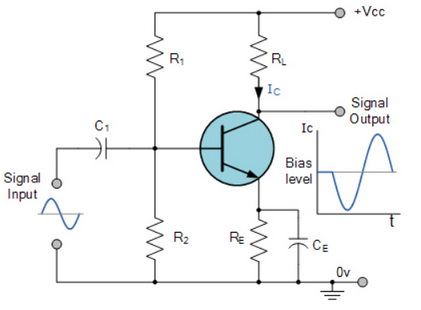
\includegraphics[width=6cm]{CircuitoAmplificadorDeUnaSolaEtapa.png} 
\caption{Circuito amplificador de una sola etapa}
\end{figure}

Este es el tipo más simple de circuito amplificador de potencia Clase A.\\
Utiliza un transistor de extremo único para su etapa de salida con la carga resistiva conectada directamente al terminal colector.\\
Cuando el transistor se "\textbf{enciende}", se hunde la corriente de salida a través del Colector, lo que resulta en una caída de voltaje inevitable a través de la resistencia del Emisor, limitando así la capacidad de salida negativa.\\
La eficiencia de este tipo de circuito es muy baja (\emph{menos del 30 porciento}) y ofrece pequeñas salidas de potencia para un gran drenaje en la fuente de alimentación de CC.\\
Una etapa de amplificador de Clase A pasa la misma corriente de carga incluso cuando no se aplica señal de entrada, por lo que se necesitan disipadores de calor grandes para los transistores de salida.

\section{Desventajas}

Su eficiencia de conversión general es muy baja ya que las grandes corrientes significan que se pierde una cantidad considerable de energía en forma de calor.\\
La eficiencia porcentual en los amplificadores se define como la potencia de salida RMS disipada en la carga dividida por la potencia total de CC tomada de la fuente de suministro como se muestra a continuación:

\begin{figure}[h]
\centering
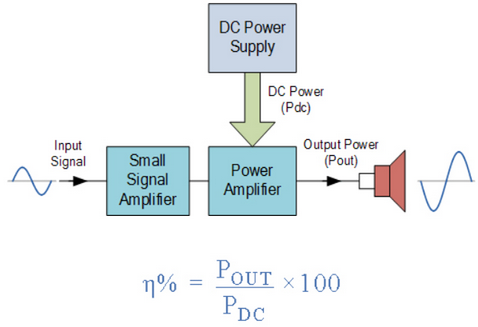
\includegraphics[width=10.5cm]{DCPOWER.png} 
\caption{conversion general}
\end{figure}

\section{Diferencia Clase A a la de Clase B}

Las diferencias de los amplificadores suelen ser muy extensas pero como las mas utilizadas son la \textbf{clase A} y \textbf{clase B} hablaremos sobre esas diferencias en su interfaz.\\
Un \emph{amplificador de potencia} funciona en \textbf{clase A} cuando la tensión de polarización y la amplitud máxima de la señal de entrada poseen valores tales que hacen que la corriente de salida circule durante todo el período de la señal de entrada.\\

\begin{figure}[h]
\centering
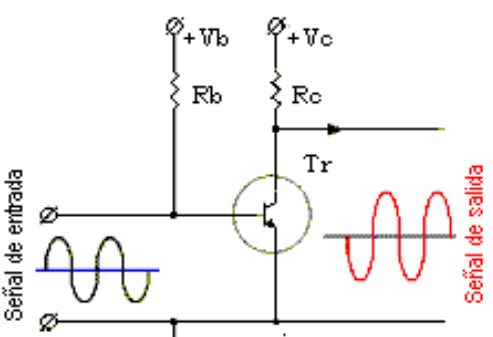
\includegraphics[width=8cm]{CLASEA.png} 
\caption{Clase A}
\end{figure}

Mientras que un \emph{amplificador de potencia} funciona en \textbf{clase B} cuando la tensión de polarización y la amplitud máxima de la señal de entrada poseen valores tales que hacen que la corriente de salida circule durante un semiperíodo de la señal de entrada.

\begin{figure}[h]
\centering
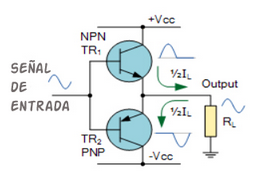
\includegraphics[width=8.5cm]{CLASEB.png}  
\caption{Clase B}
\end{figure}

Para la operación de Clase B, se utilizan dos transistores de conmutación complementarios con el punto Q (que es su punto de polarización) de cada transistor ubicado en su punto de corte. Esto permite que un transistor amplifique la señal más de la mitad de la forma de onda de entrada, mientras que el otro transistor amplifica la otra mitad.

\end{document}
